\documentclass[12pt]{article}

%% Je suis francophone !

\usepackage[english]{babel}


%% Je veux pouvoir inclure des figures...
\usepackage[pdftex]{graphicx}

%% ... des figures ``jpeg'' ou ``pdf'' ou "png"
\DeclareGraphicsExtensions{.jpg,.pdf,.png}

%% Je veux pouvoir inclure gantt diagram...
\usepackage{pgfgantt}

%% Je veux créer des Hyperdocuments
\usepackage[pdftex,colorlinks=true,linkcolor=blue,citecolor=blue,urlcolor=blue]{hyperref}

%% Je contrôle la taille de ma zone imprimée...
\usepackage{anysize}
%% ...en définissants les marges {gauche}{droite}{haute}{basse}
\marginsize{18mm}{18mm}{12mm}{12mm}

%% J'inclue une bibliographie ; j'ai donc besoin du package natbib
\usepackage{natbib}

%Pour utiliser la virgule comme séparateur décimal en mode math,
%sans que Latex introduise un espace inutile après la virgule :
\usepackage{icomma}


\usepackage{minted}

%% pour les referneces
\usepackage{url}


\usepackage{afterpage}

\usepackage{a4wide}
\usepackage{csquotes}
\usepackage{amsmath,amssymb}
\usepackage{bm}
\UseRawInputEncoding
\usepackage[toc,page]{appendix}
\usepackage{color}
\usepackage{captcont}
\usepackage{hvfloat}
\usepackage{siunitx}
\usepackage{forest}
\renewcommand{\figurename}{Fig.}
\usepackage{indentfirst}
\setlength{\parindent}{1cm}

%%\MakeOuterQuote{"}
\oddsidemargin0cm

\topmargin-2cm     %I recommend adding these three lines to increase the 
\textwidth16.5cm   %amount of usable space on the page (and save trees)
\textheight23.5cm 
\usepackage{setspace}
\usepackage[margin=20mm,labelfont=bf]{caption}
\usepackage[left=20mm, right=20mm, top=20mm, bottom=20mm]{geometry}
\usepackage{amssymb}
\usepackage[section] {placeins}
\usepackage{verbatim}
\usepackage{wrapfig}
\usepackage{mwe,tikz,pgfplots}

%% pour les codes 
\usepackage{listings}

\newcommand{\vect}[1]{\hat{\boldsymbol{#1}}}
\title{Report V1}
\author{Congo Job}
\usepackage{minted}
\begin{document}
    \maketitle

\tableofcontents

\section{Introduction}
La pratique régulière d’activités physiques comporte de nombreux bénéfices tel 
qu' une amélioration de la santé mentale ,la prévention des maladies cardiovasculaire , limiter la prise  de poids et bien d'autres . 

Cependant, on observe un déclin de la pratique d’activités physiques.
il apparaît primordia d’encourager les jeunes à maintenir une activité physique ou devenir plus actif , c'est dans cette optique que s'inscrit ce projet . 



\subsection{Sport et sciences sociales}

Créée en 1979 par Bernard Michon à Strasbourg ,l’unité de recherche Sport et sciences sociales
demeure la seule unité de recherche STAPS du Grand Est et est reconnue comme une structure de recherche incontournable  en sciences sociales du sport dans le paysage français et européen.
Regroupant plus de 20 chercheurs (titulaires et associés) et 17 doctorants, elle réalise  des	ouvrages	et	des	articles de	référence (plus	de	174	publications).




\subsection{Main Objectives}

L'objectif de ce travail est d'identifier des profils de praticiens basés sur des qualificatifs positifs ou négatifs, c'est-à-dire d'attribuer un profil à chaque cluster des données et d'estimer la force de ces profils, c'est-à-dire le nombre de clusters ou de profils qui sont les plus représentatifs des données.


\subsection{Specific Objectives}
Nous allons d'abord effectuer un prétraitement des données par la renormalisation des données , la suppression des valeurs aberrantes,  compléter ou  supprimer les valeurs manquantes, puis pour analyser les données nous utiliserons différents algorithmes tels que : K-means, analyse en composantes principales, arbres de décision. Enfin, nous testerons la solidité de notre cluster en utilisant des algorithmes de classification tels que : la régression logistique, les k- plus proches voisins,...



Le diagramme de Gantt ci-dessous nous donne un aperçu rapide de l'organisation du travail dans le temps .

\begin{ganttchart}[
  hgrid,x unit=1.5mm,
  hgrid style/.style={draw=black!5, line width=.75pt},
  vgrid={*{6}{draw=none},dotted},
  time slot format=little-endian,
]{1-04-2022}{27-05-2022}
  \gantttitlecalendar{ month=shortname,week=4} \\
  \ganttgroup{Report V0}{1-04-2022}{5-04-2022}\\
  \ganttbar{data pre-processing}{5-04-2022}{30-04-2022}\\
  \ganttbar{clustering methods}{5-04-2022}{10-05-2022}\\
  \ganttbar{Validation}{5-04-2022}{22-05-2022}\\
  \ganttgroup{Report V1}{5-04-2022}{22-05-2022}\\
  \ganttbar{data pre-processing}{5-04-2022}{30-04-2022}\\
  \ganttbar{clustering methods}{5-04-2022}{10-05-2022}\\
  \ganttbar{Validation}{5-04-2022}{22-05-2022}\\
  \ganttgroup{Report Vfinale}{22-05-2022}{27-05-2022}\\
\end{ganttchart}



\section{Description of raw data}

Le dataset contient des informations personnels sur les lycéens ( 1070 participants )tel  que leur initial, le Lycée, le sexe , le choix d'étude ,le travail des parents et le support des parents ainsi que la date de naissance , la  morphologie de la personne ( la taille et le poids ) . Une vingtaine des  variables mesurent la nature de la motivation par exemple la jouissance , l'affiliation , la condition physique  et  le dégré de motivation tel que SIMS intrinsic et SIMS external regulation . 

Enfin le reste des  variables (71)  recolté de  la manière suivante :
On pose une question : "En EPS, quel est le sport que vous avez le plus apprécié ?".

Puis on lui indique :
"Nous allons maintenant te présenter des mots qui vont te permettre de décrire ton ressenti par rapport à ce sport. Votre travail consiste à indiquer, le plus rapidement possible, si vous êtes d'accord ou non avec ces propositions en cliquant sur oui ou non.
Le temps de réponse a été pris en compte dans chaque réponse. Si ce temps est court, cela signifie que le terme semble évident.
Par exemple, si le sport est "le football", l'élève pourra répondre "oui" rapidement au qualificatif "plaisir", "non" rapidement au qualificatif "beauté".

Les réponses possibles à chaque question sont "oui", "non", "je ne sais pas". Lorsque la réponse à une question est "oui", la valeur du temps est positive, négative dans le cas de "non" et zéro dans le cas de "je ne sais pas".


\begin{figure}[h]
\begin{center}
\includegraphics[scale=0.5]{donnée_brute.png} 
\caption[]{ Raw \ data}
\end{center}
\end{figure}


\section{Preprocessing}

\subsection{Preprocessing Method}

Les valeurs manquantes sont mis à zéros en supposant que le qualificatif n'intéresse pas les étudiants concernés et qu'ils auraient pu  répondre : "je ne sais pas".
Pour la gestion des valeurs aberrantes , celles qui sont  supérieur à 5*écart-type ont été mise à zéros en fin de ne pas impacter le poids donnée à chaque  mot. L'écart-type est calculé en utilisant les données non signées dans le but de réduire les valeurs extrême et éviter la possible compensation des valeurs.
Les étudiants ayant répondu "je ne sais pas" à toutes ces questions n'ont pas été considéré dans la suite du projet .  
La normalisation est faite par ligne dans le but de conserver ce qui est "important" pour chaque personne. 




\subsection{Results of processed data}

\begin{figure}[h]
\begin{center}
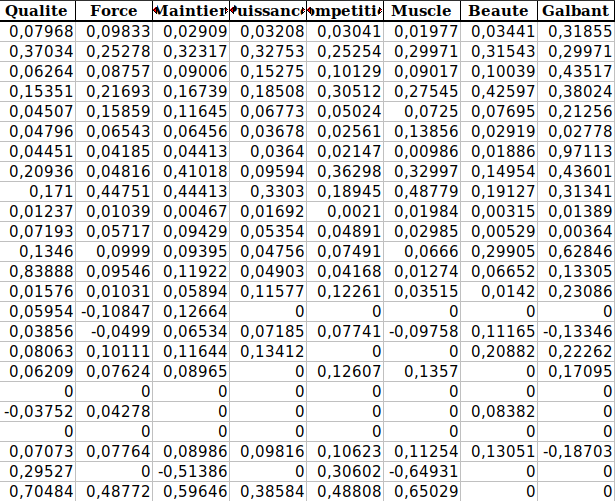
\includegraphics[scale=0.7]{donnée_nettoyé.png} 
\caption[]{Data \ processed }
\end{center}
\end{figure}



Les mots les plus "importants"  et les moins "importants" pour chaque personne sont respectivement proche de soit 1 ou de -1 . Ceux qui  sont  moins "importants" sont proches de zero.

Le jeu de données nettoiyée contient 1050
lycéens et 71 caractéristiques.


\section{Clustering} 


\subsection{Principal component analysis}

L'analyse en composantes principales (ACP) est utilisé pour réduire la dimension des données en quelques variables et garder les données les plus importants. C'est une méthode de la statistique multivariée, qui consiste à transformer des variables liées entre elles (dites « corrélées » en statistique) en nouvelles variables decorrélées les unes des autres. 

Pour déterminer le nombre de composante optimale , la comande fviz\_eig de Rstudio, a été solicité. Cette fonction permet d'avoir le graphique des valeurs propres.


Les valeurs propres mesurent la quantité de variance expliquée par chaque axe principal. Elles sont grandes pour les premiers axes et petites pour les axes suivants.


\begin{figure}[H]
\begin{center}
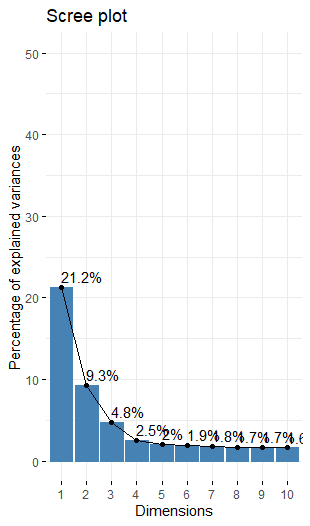
\includegraphics[scale=1.4]{ACP_1.png} 
\caption[]{\ }
\end{center}
\end{figure}

D'après le graphique ci-dessus, nous pourrions vouloir nous 
arrêter à la cinquième composante principale  car la variation est moindre après la cinquième.
Cependant 39.79760 \% des informations (variances) contenues
dans les données sont retenues par les 5  premières composantes principales.


Les graphique ci-dessous montre le top 30 des variables contribuant le plus aux 5 composantes principales. 
Les lignes en pointillé rouge, sur les graphiques, indique  la valeur  contribution moyenne.
 

\begin{figure}[H]
\begin{center}
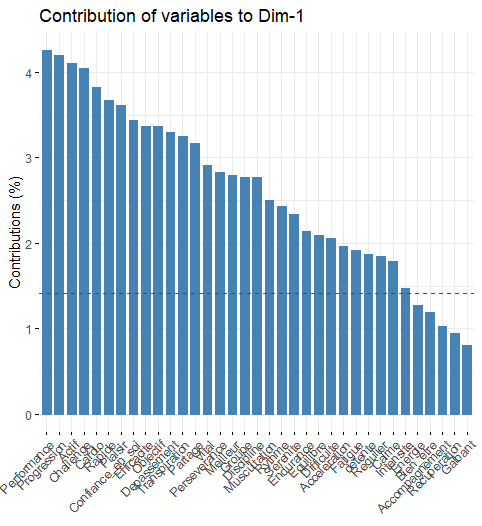
\includegraphics[scale=1.3]{ACP_2.png} 
\caption[]{\ }
\end{center}
\end{figure}


\begin{figure}[H]
\begin{center}
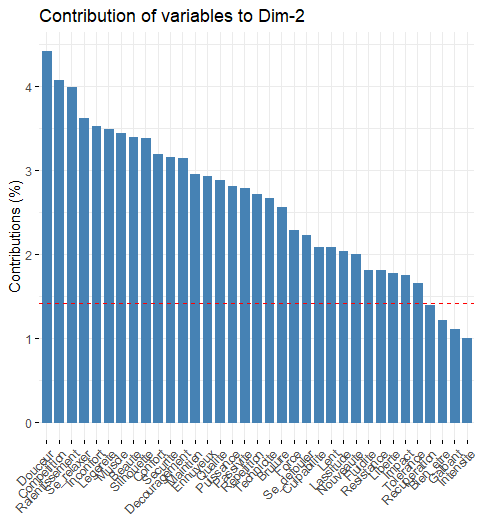
\includegraphics[scale=1.3]{ACP_3.png} 
\caption[]{\ }
\end{center}
\end{figure}


\begin{figure}[H]
\begin{center}
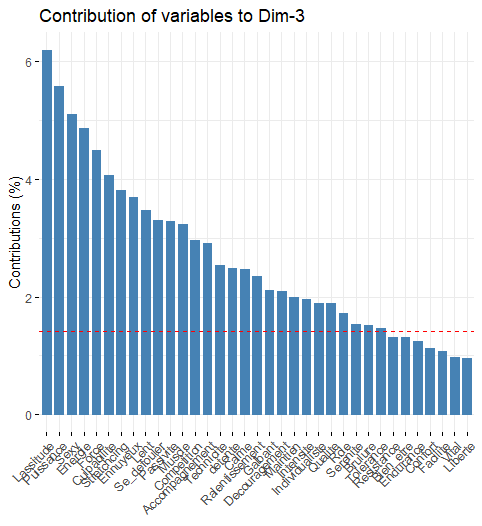
\includegraphics[scale=1.3]{ACP_4.png} 
\caption[]{\ }
\end{center}
\end{figure}


\begin{figure}[H]
\begin{center}
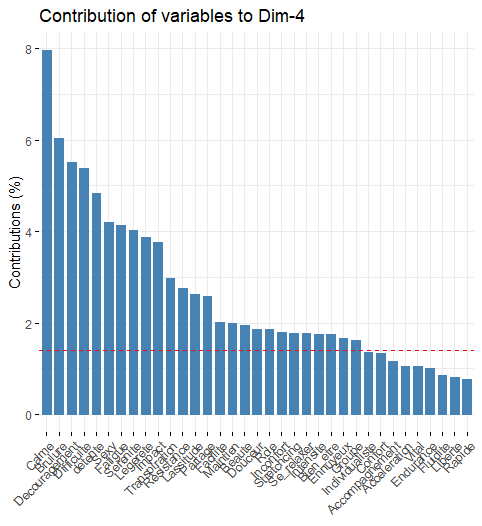
\includegraphics[scale=1.3]{ACP_5.png} 
\caption[]{\ }
\end{center}
\end{figure}


\begin{figure}[H]
\begin{center}
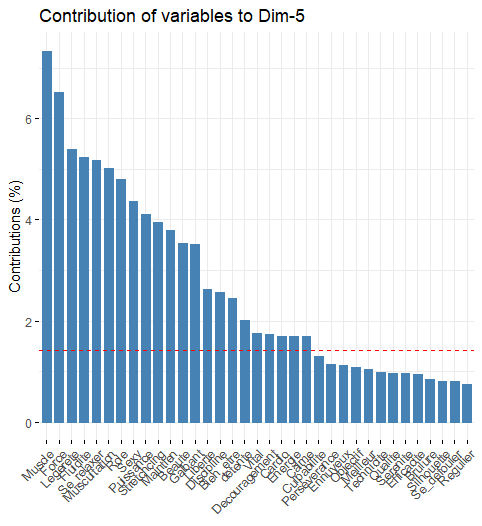
\includegraphics[scale=1.3]{ACP_6.png} 
\caption[]{\ }
\end{center}
\end{figure}

Les variables les moins importants  sont les suivantes : "Recuperation" et  "Facilité".

\newpage   


\subsection{Hierarchical Clustering on Principal Components} 
Pour réaliser le clustering, nous allons utilisé  Hierarchical Clustering on Principal Components( HCPC).
Cette méthode permet de combiner les trois méthodes standards utilisées dans les analyses de données multivariées :

\begin{itemize}
    \item  Méthodes en composantes principales (PCA, CA, MCA, FAMD, MFA),
    \item  Regroupement hiérarchique et 
    \item  Clustering de partitionnement, en particulier la méthode des k-moyennes.
\end{itemize}

\vspace{0.2 cm}

L'algorithme de la méthode HCPC a 4 principales étapes :

\begin{itemize}
    \item{1)} Effectue une ACP. Choisisse le nombre de dimensions à retenir en spécifiant l’argument ncp. Dans notre cas ,la  valeur est 5.
    \item{2)} Applique la classification hiérarchique sur le résultat de l’étape 1.
    \item{3)} Choisisse le nombre de groupes en fonction du dendrogramme obtenu à l’étape 2. Un partitionnement initial est effectué.Dans notre cas ,la  le nombre de groupes est 3.
    \item{4)} Effectue le k-means pour améliorer le partitionnement initiale obtenu à l’étape 3.
\end{itemize}



Voici les lignes de codes principales pour :


\begin{lstlisting}

res.pca <- PCA(data_base , ncp = 5 ,graph = TRUE)
res.hcpc <- HCPC(res.pca,nb.clust=3,consol=FALSE,graph=TRUE)

plot(res.hcpc,choice = "tree")
plot(res.hcpc,choice = "map", draw.tree = FALSE)
plot(res.hcpc,choice = "3D.map")
catdes(res.hcpc$data.clust,ncol(res.hcpc$data.clust))

\end{lstlisting}

\begin{figure}[H]
\begin{center}
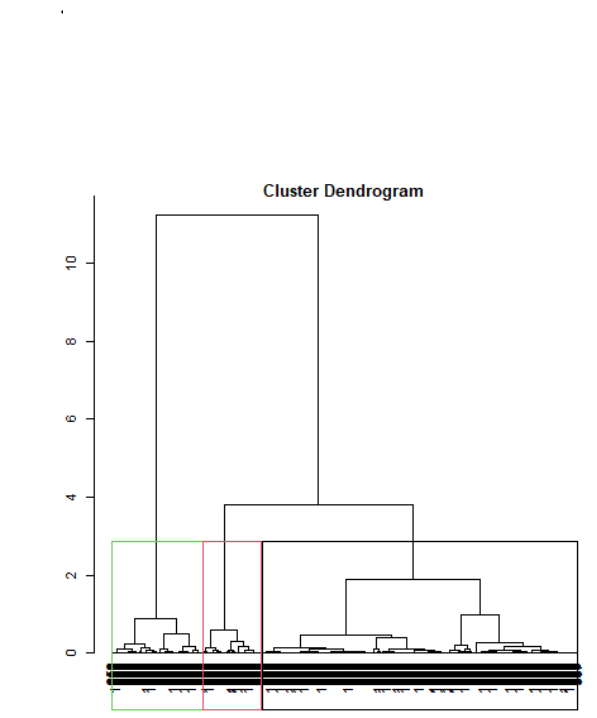
\includegraphics[scale=0.65]{classification_1.png} 
\caption[]{Hierarchical \ tree}
\end{center}
\end{figure}


\begin{figure}[H]
\begin{center}
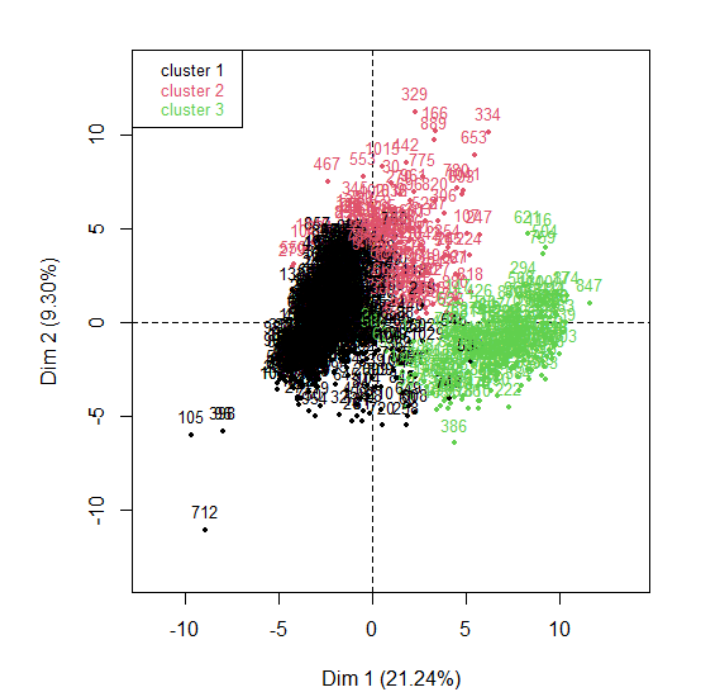
\includegraphics[scale=0.7]{classification_2.png} 
\caption[]{Ascending \ Hierarchical \ Classification \ of \ the \ individuals }
\end{center}
\end{figure}

\begin{figure}[H]
\begin{center}
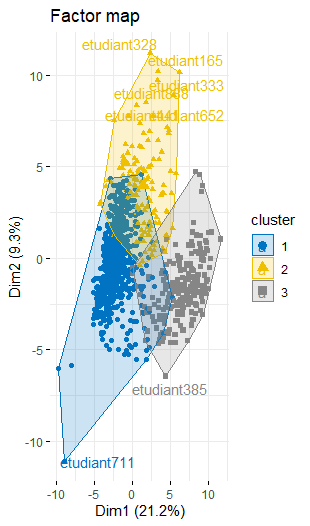
\includegraphics[scale=0.8]{hcpc.png} 
\caption[]{Ascending \ Hierarchical \ Classification \ of \ the \ individuals }
\end{center}
\end{figure}


\subsection{Results of HCHC} 

Le cluster 1 est constitué d'individus partageant :

- des valeurs élevées pour les variables Galbant, Culpabilite, Ennuyeux, 
Stretchcing, Securite, Decouragement, Ralentissement, Lassitude,
Inconfort et Passivite (les variables sont triées à partir des plus fortes).

- des valeurs faibles pour des variables comme Progression, Transpiration, Performance,
Actif, Challenge, Plaisir, Objectif, Persévérance, Confiance en soi et Cardio 
(les variables sont triées à partir des plus faibles).


Le cluster 2 est constitué d'individus partageant :


- des valeurs élevées pour des variables comme Se défouler, Puissance, Compétition, Technicité, Qualite, Energie, Confort, Muscle, Force et Intensite (les variables sont triées à partir des plus fortes).

- des valeurs faibles pour les variables Sexy, Meilleur, Calme et Vital (les variables sont triées à partir des plus faibles).


Le cluster 3 est constitué d'individus partageant :


- des valeurs élevées pour des variables comme Progression, Actif, Performance, Challenge, Cardio, Partage, Plaisir, Depassement, Rapide et Efficacite (les variables sont triées à partir des plus fortes).

- des valeurs faibles pour des variables telles que Confort, Securite, Galbant, Douceur, Ennuyeux, Force, Maintien, Qualite, Beauté et Inconfort (les variables sont triées à partir des plus faibles).


\section{Classification}  %%%%  Testing the strength of clusters %%%%
 
 Nous avons séparer nos données en 3 parties :
- 80 \% des données pour le choix de l'algorithme de sélection .
- 20 \% des données pour tester le modele finale et éventuellement sélectionner les colonnes les plus importantes.

\subsection{Choice of Classification algorithm} 

 4 classificateurs multi-classes sont utilisés : le classificateur à vecteurs de soutien
(SVC), classificateur à vecteur de support linéaire
(LSVC), k-nearest neighbors (KNN) et régression logistique (logreg). 
(KNN) et régression logistique (logreg).

voici le graphique de la  performance de chaque modèle : 


\begin{figure}[H]
\begin{center}
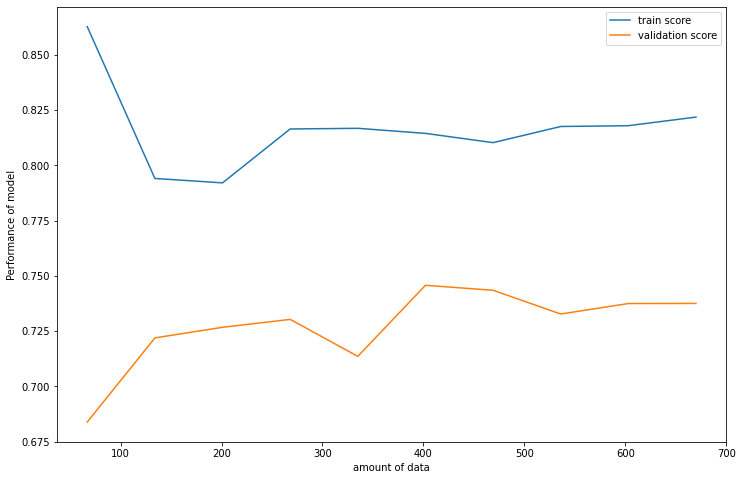
\includegraphics[scale=0.6]{learning_curve_1.png} 
\caption[]{ KNN \ learning \ curve }
\end{center}
\end{figure}

\begin{figure}[H]
\begin{center}
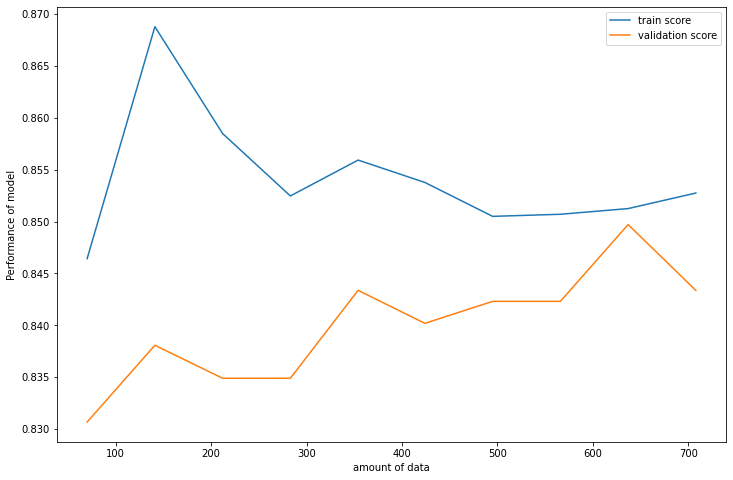
\includegraphics[scale=0.6]{learning_curve_2.png} 
\caption[]{ logreg \ learning \ curve }
\end{center}
\end{figure}

\begin{figure}[H]
\begin{center}
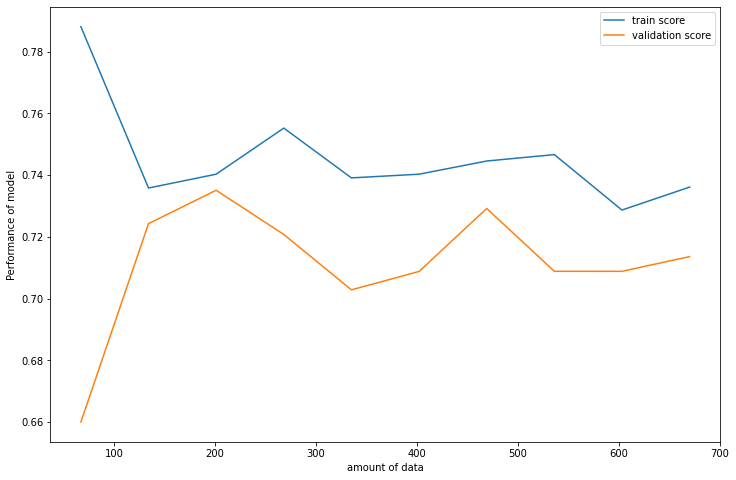
\includegraphics[scale=0.6]{learning_curve_3.png} 
\caption[]{ LSVC \ learning \ curve }
\end{center}
\end{figure}

\begin{figure}[H]
\begin{center}
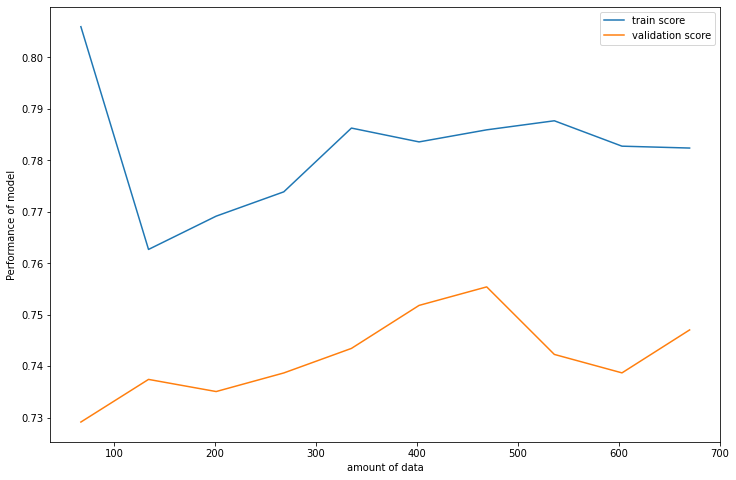
\includegraphics[scale=0.6]{learning_curve_4.png} 
\caption[]{ SVC \ learning \ curve }
\end{center}
\end{figure}


D'après les graphiques ci- dessous , la performance ou modele de lostigic Regression et SVC soit plus stable et meilleur que les autres modèles. On peut dire que les deux modèle ne sont pas en overfiting
(score train et score val sont proches) contrairement aux 2 autres.


Nous avons utlisé  GridSearchCV pour optimser les hyperparametres du modele  logistic Regression. 
GridSearchCV nous permet de les meilleurs hyperpametre en comparant les différents performances 
 de chaque combinaison grâce a la technique de cross-validation.

La cross-validation consiste découper le jeu de données en k parties égales  ( ici k = 5). Tour à tour, chacune des k parties est utilisée comme jeu de test. Le reste (autrement dit, l’union des k-1 autres parties) est utilisé pour l'entraînement.

  
\subsection{Feature selection} 

Le graphique ci- dessous nous montre la variance de chaque features. 
 4 candidats  le seuil se demarquent : 0.8 , 0.06 , 0.04 et 0.02.


\begin{figure}[H]
\begin{center}
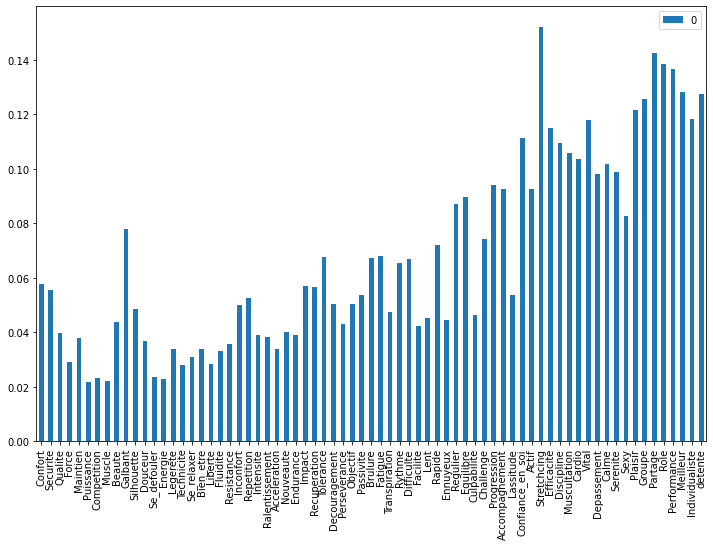
\includegraphics[scale=0.6]{barlot.png}
\caption[]{ variance\ of \ each \ features}
\end{center}
\end{figure}

Pour éliminer les valeurs inférieur à ce seuil , La fonction VarianceThreshold de scikit-learn est utilisé.

Au final, le seuil fixé à 0.02 donne de meilleurs résultats. Aucun  colonne n'a été suprimée . 

\subsection{Results final model} 

\begin{figure}[H]
\begin{center}
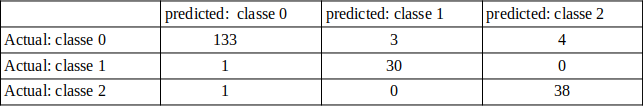
\includegraphics[scale=0.6]{confusion_matrix_1.png} 
\caption[]{  confusion \ matrix }
\end{center}
\end{figure}



\begin{figure}[H]
\begin{center}
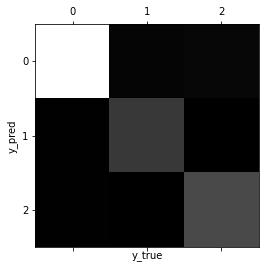
\includegraphics[scale=0.6]{confusion_matrix_2.png} 
\caption[]{confusion \ matrix}
\end{center}
\end{figure}


Nous obtenons des résultats satisfaisant : 
seulement 9 valeurs mal placées , la valeur de 0.964 et  0.94768 pour le recall\_score et le f1\-score.


\section{Conclusion}
L'objectif principal du projet était de faire du  clustering sur nos données.
Grace au clustering HCPC , nous pouvons distinguer 3 types d'étudiants :

\begin{itemize}

\item les démotivés , ceux qui recherchent le bien-être et la simplicité dont certaines variables caractéristiques du cluster sont :  Culpabilite, Ennuyeux,  Decouragement, Ralentissement, Inconfort 

 \item Dans le deuxième groupe , on a ceux qui aiment les sports de combat comme la lutte, la boxe le MMA. il est caractérisé par ses mots : Puissance, Competition, Technicite, Qualite, Energie, Muscle, Force and Intensite 

 \item Le dernier groupe  se distingue par ses mots : Progression, Performance, 
Challenge, Cardio, Partage, Depassement, Rapide and Efficacite. 
On retrouve ceux qui apprécient la course à pied et les activité de nature . 

\end{itemize}

En ce qui concerne la classification ,L'un des meilleur algorithme (SVM) a donné la valeur 0.9549 de précision, 0.9 de rappel et 0.9255 de f1-score.(Par contre, l'ensemble de données de ce projet n'est pas assez grand.)

\begin{thebibliography}{9}

\bibitem{text}
\url{https://www.cairn.info/revue-staps-2018-2-page-99.htm}

\bibitem{text}

\url{https://solidarites-sante.gouv.fr/prevention-en-sante/preserver-sa-sante/article/activite-physique-et-sante}

\bibitem{text}
\url{https://e3s.unistra.fr/equipe/presentation/}

\bibitem{text}
\url{https://scikit-learn.org}

\bibitem{}
\url{https://fr.wikipedia.org/wiki/Analyse_en_composantes_principales}


\bibitem{text}
\url{http://www.sthda.com/english/}

\bibitem{text}
\url{http://www.sthda.com/english/articles/31-principal-component-methods-in-r-practical-guide/117-hcpc-hierarchical-clustering-on-principal-components-essentials/#algorithm-of-the-hcpc-method}


\bibitem{text}
\url{https://husson.github.io/teaching.html}


\bibitem{text}
\url{https://www.youtube.com/c/MachineLearnia}

\bibitem{text}
\url{}

\end{thebibliography}



\end{document}

